\section{Simulation}\label{sec:Simulationsresultate}

Für das Testen des theoretischen Aufbaus der Yagi-Antenne wurde eine Simulation mit \textit{CST Studio Suite} durchgeführt. Somit kann vor dem Zusammenbau der Antenne dessen Funktion verifiziert werden und falsche Berechnungen überprüft werden. Dieser Abschnitt erläutert die Vorgehensweise bei der Simulation und dessen Resultate.

\subsection{Aufbau der Antenne}

Um die Antenne so realitätsnahe wie möglich simulieren zu können wurde Aluminium ($\sigma = $ \SI{3.56e+7}{S/m}) und Holz aus der Materialbibliothek geladen. Anschliessend wurde die Antenne anhand den Parametern aus Kapitel \ref{sec:Berechnung} konstruiert. Die fertig konstruierte Antenne ist in Abbildung \ref{fig:Simulation_Yagi} zu sehen.

\begin{figure}[h!]
	\centering
	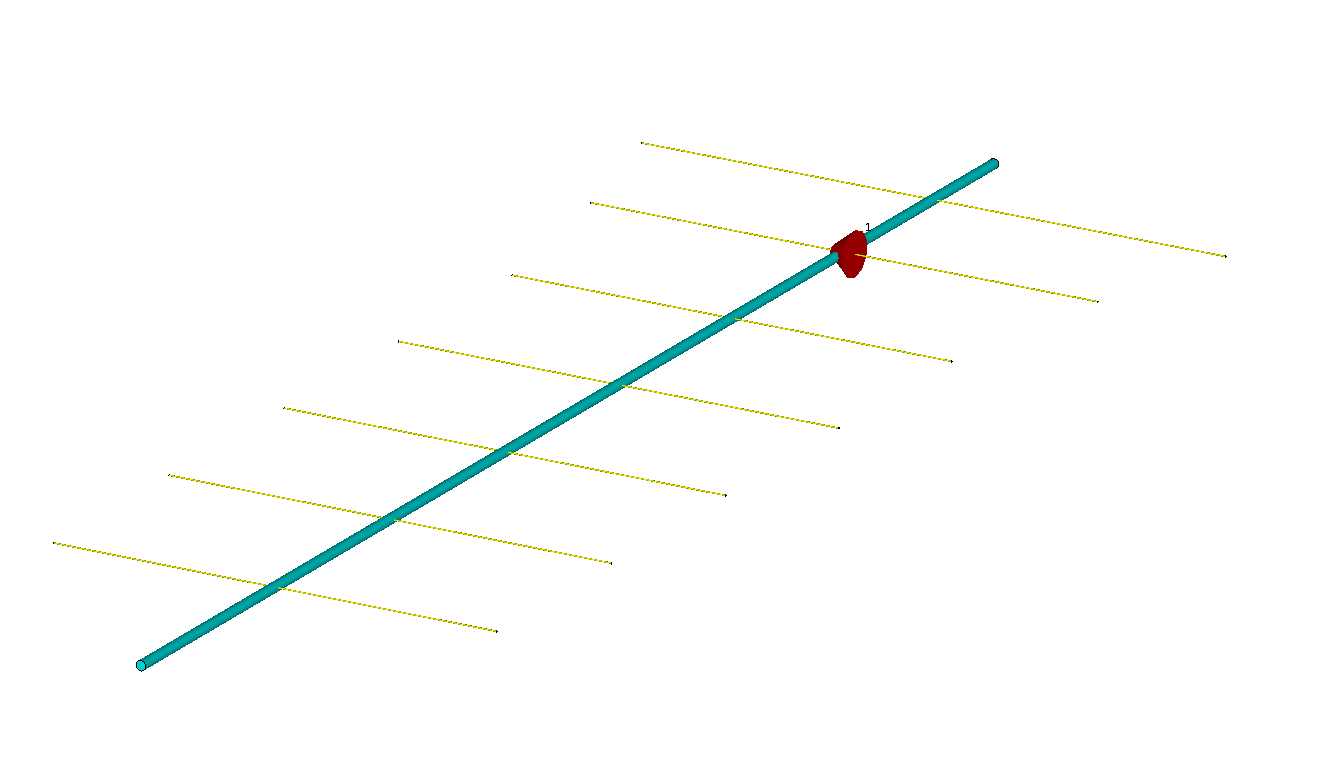
\includegraphics[width=\textwidth]{Yagi.png}
	\caption{Aufbau der Yagi-Antenne in \textit{CST Studio Suite}.}
	\label{fig:Simulation_Yagi}
\end{figure}

\subsection{Simulationsresultate}

Für die Simulation sind für den Bericht vor allem zwei Parameter wichtig: die S-Parameter und das Fernfeld. Letzteres wurde bei \SI{144}{MHz} gemessen und ist in Abbildung \ref{fig:Simulation_Yagi_Fernfeld} zu sehen. Zur Veranschaulichung ist ein 3D-Diagramm zu sehen, wie bereits in Abbildung \ref{fig:yagi} dargestellt. Daneben befindet sich das Richtdiagramm, welches im Bericht von \textit{hf1} ausführlich beschrieben ist. Aus dem Richtdiagramm lässt sich eine Halbwertsbreite von \SI{56.0}{\degree} und eine Abstrahlstärke in Hauptrichtung von \SI{10.3}{dBi} ablesen.

 \newpage

\begin{figure}[h!]
	\centering
	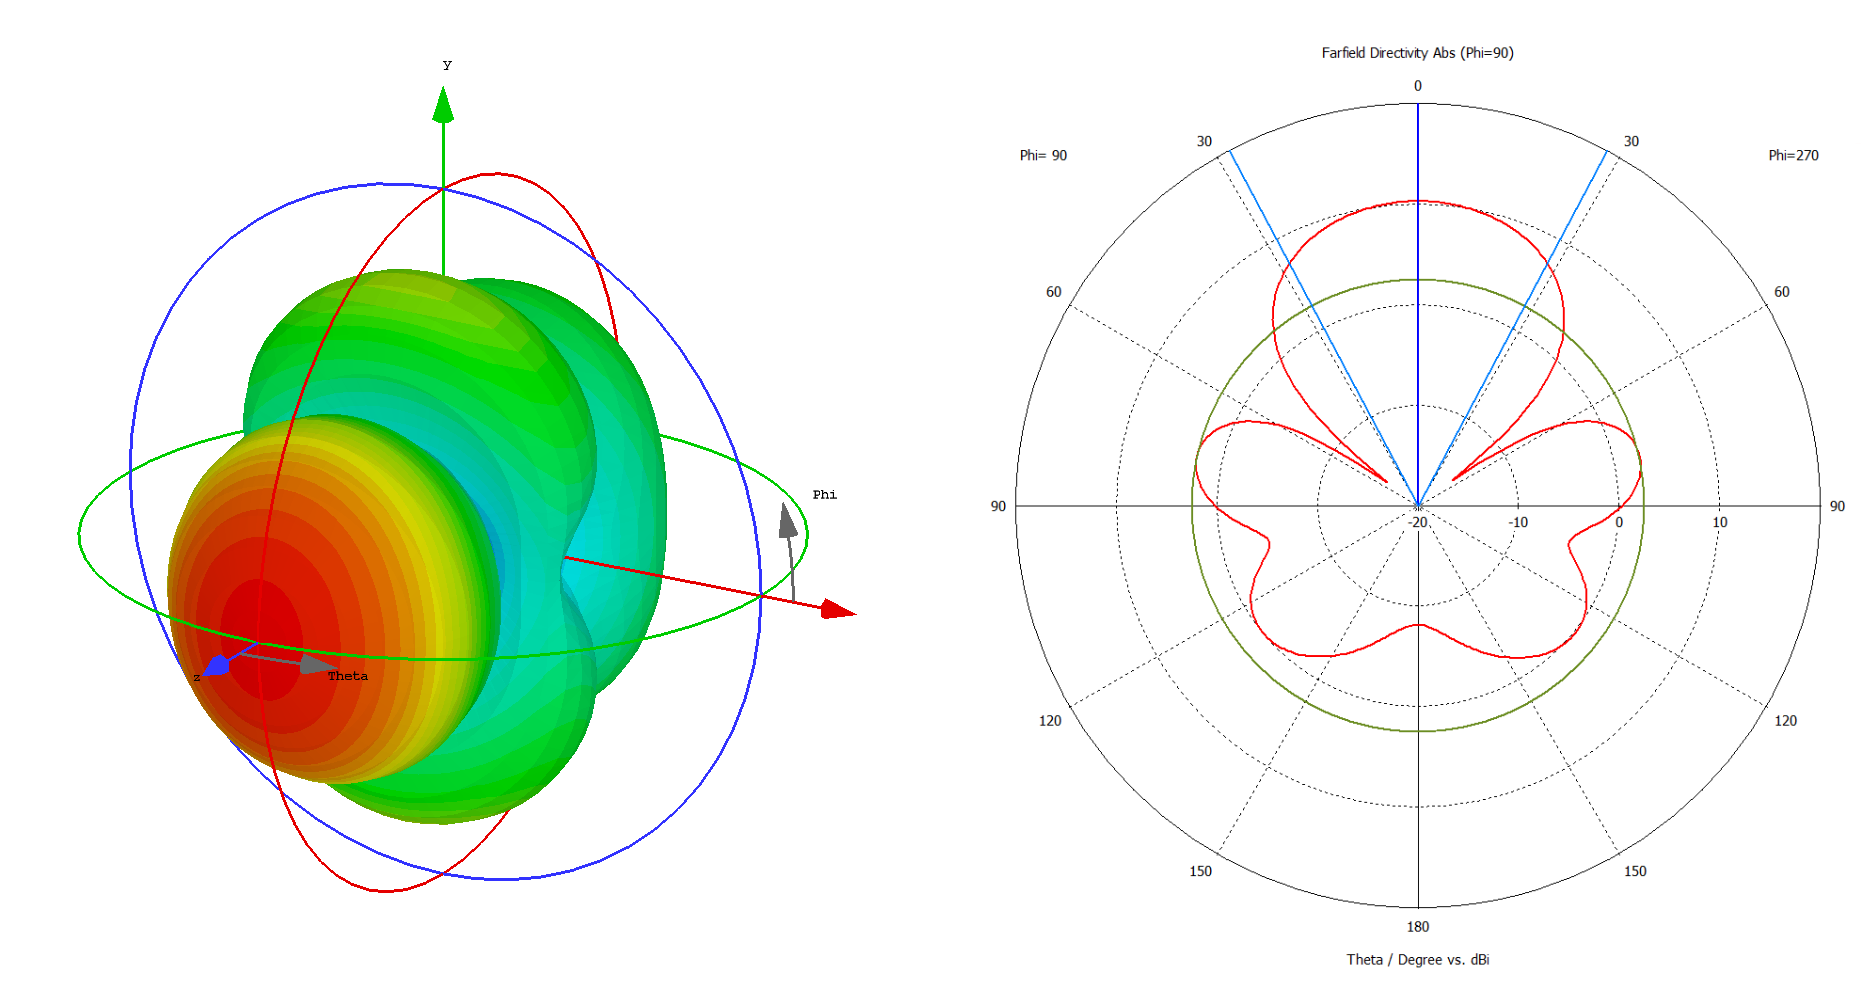
\includegraphics[width=\textwidth]{Yagi_Fernfeld.png}
	\caption{Fernfeld 3D- und Richtdiagramm der Yagi-Antenne.}
	\label{fig:Simulation_Yagi_Fernfeld}
\end{figure}

Als Vergleich wurden eine Messung mit nur zwei Direktoren durchgeführt. Die identische Simulation wurde nochmals laufen gelassen, wobei sich das 3D- und Richtdiagramm aus Abbildung \ref{fig:Simulation_Yagi_Fernfeld_2dir} ergibt. Hierbei ist bereits ersichtlich, dass die Hauptkeule viel breiter ist und sich total weniger Keulen ergeben. Die Halbwertsbreite beträgt bei dieser Antenne \SI{89.2}{\degree} und die Abstrahlstärke in Hauptrichtung \SI{7.6}{dBi}. Somit kann bestätigt werden, dass mehr Direktoren zu einer kleineren Halbwertsbreite führen und dessen Abstrahlstärke dadurch auch stärker wird.

\begin{figure}[h!]
	\centering
	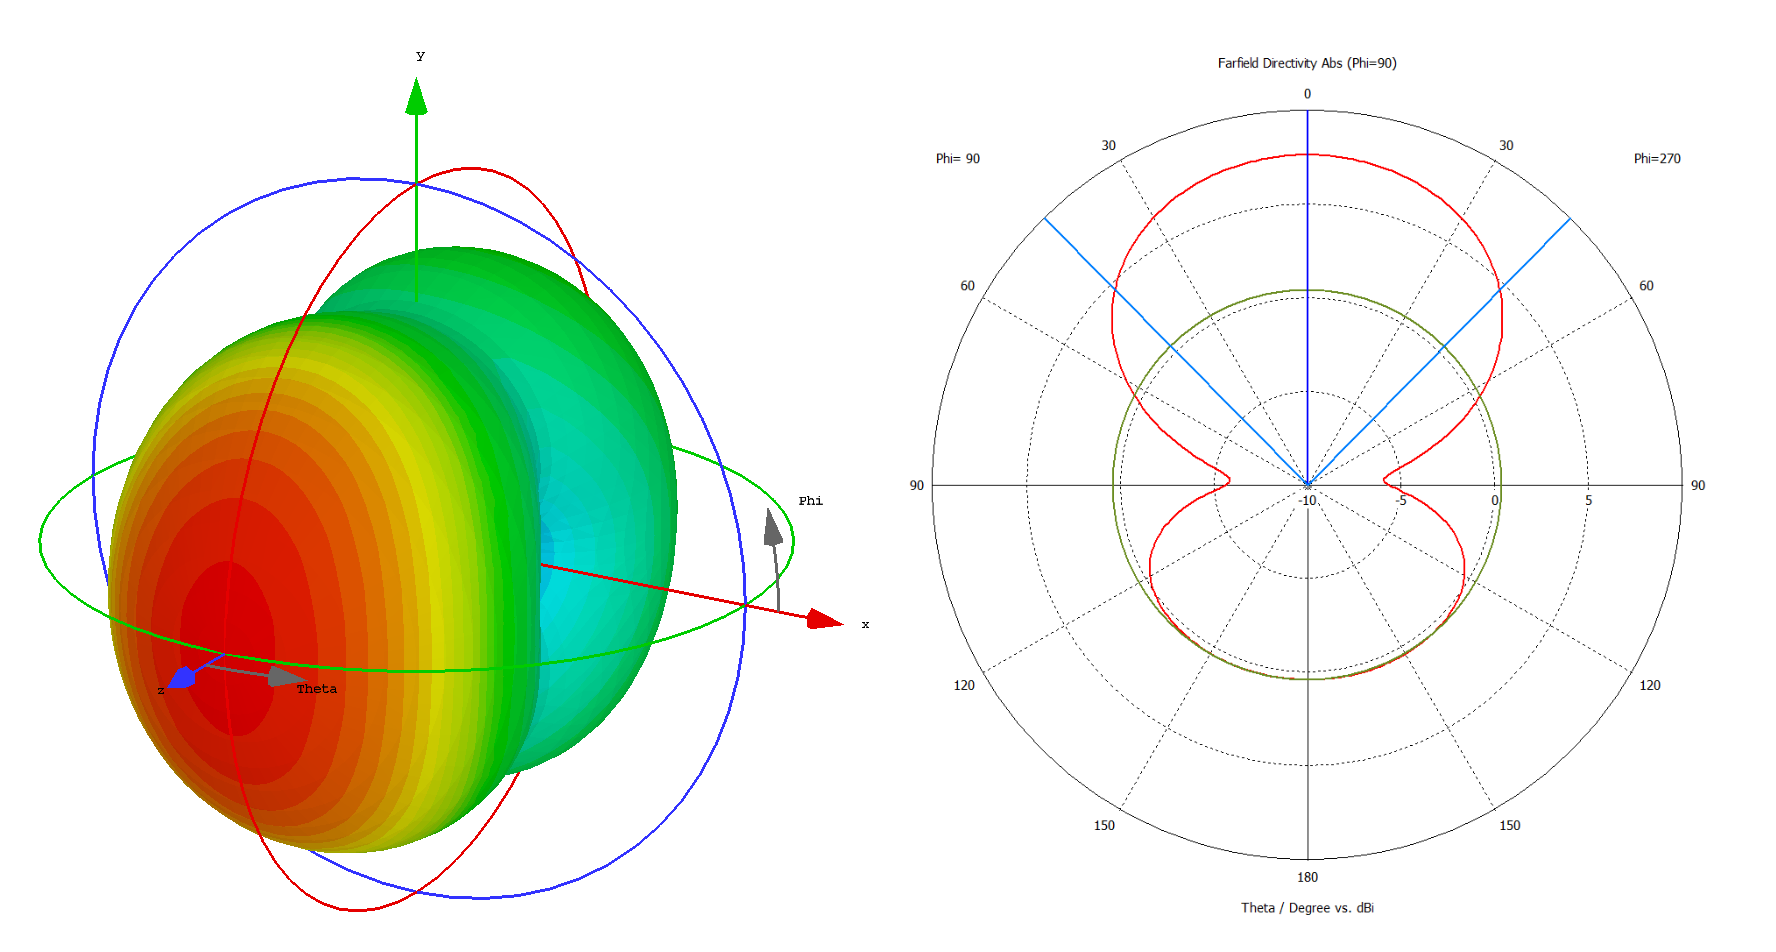
\includegraphics[width=\textwidth]{Yagi_Fernfeld_2dir.png}
	\caption{Fernfeld 3D- und Richtdiagramm der Yagi-Antenne mit nur 2 Direktoren.}
	\label{fig:Simulation_Yagi_Fernfeld_2dir}
\end{figure}

\newpage

Während sich die 3D-Diagramme gut für das Verständnis der Abstrahlung der Antenne eignen, sind für den Bericht  die Messungen bezüglich der S1,1 Parameter aussagekräftiger (und vor allem auch einfacher messbar). Diese Parameter werden anschliessend in Kapitel \ref{sec:Messung} im Labor gemessen und können als Verifikation verwendet werden. Somit wurde die Antenne mit dem \textit{Frequency Domain Solver} ausgemessen.

\begin{figure}[h!]
	\centering
	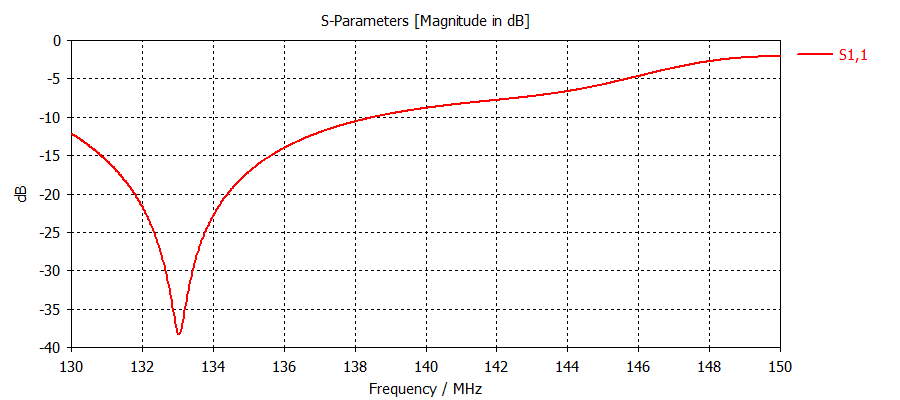
\includegraphics[width=\textwidth]{result.png}
	\caption{S1,1 Parameter der simulierten Yagi-Antenne.}
	\label{fig:Simulation_result}
\end{figure}

Abbildung \ref{fig:Simulation_result} zeigt die S1,1 Parameter der konstruierten Yagi-Antenne. Wie bereits erwähnt wurde diese für \SI{144.125}{MHz} berechnet, wobei bei der Simulation eine Grenzfrequenz von exakt \SI{133.0}{MHz} gemessen wird. Die dabei abweichende Grenzfrequenz kann vor allem durch das Anpassen der Länge des Dipols verbessert werden. Für das bessere Verständnis der Antenne werden die für die Simulation berechneten Parameter um $\pm$ \SI{5}{cm} angepasst, womit dessen Auswirkungen auf die S1,1 Parameter dargestellt werden können.

\begin{figure}[h!]
	\centering
	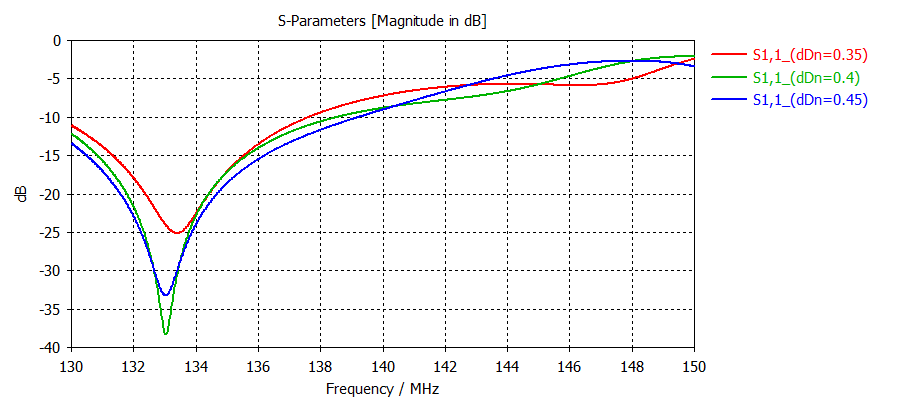
\includegraphics[width=\textwidth]{dDn.png}
	\caption{Resultat der S1,1 Parameter durch Abändern von $d_\mathrm{Dn}$.}
	\label{fig:Simulation_dDn}
\end{figure}

In Abbildung \ref{fig:Simulation_dDn} wird das Resultat durch verändern des Abstandes zwischen den Direktoren dargestellt. Erwartungsgemäss hat dieser Abstand nahezu keinen Einfluss auf die Grenzfrequenz, sondern nur auf den Antennengewinn. Kleine Abweichungen vom berechneten Wert können dabei bereits eine Verschlechterung von \SI{15}{dB} ausmachen (dies liegt jedoch auch daran, dass alle 5 Direktoren dabei voneinander um \SI{5}{cm} verschoben werden, weshalb der letzte Direktor ganze \SI{25}{cm} weiter hinten liegt).

\begin{figure}[h!]
	\centering
	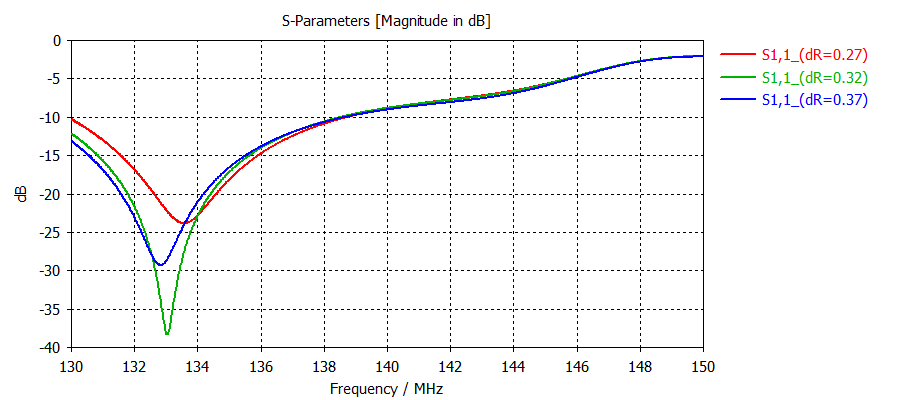
\includegraphics[width=\textwidth]{dR.png}
	\caption{S1,1 Parameter mit sich änderndem Abstand des Reflektors zum Dipol.}
	\label{fig:Simulation_dR}
\end{figure}

Auch ein Abändern des Abstandes des Reflektors zum Dipol hat nur einen minimalen Einfluss auf die Grenzfrequenz. Dies ist der Abbildung \ref{fig:Simulation_dR} zu entnehmen. Dabei haben die kleinen Veränderungen nahezu das selbe Ausmass wie bei den Direktorenabständen in Abbildung \ref{fig:Simulation_dDn}. Das Verhalten der S1,1 Parameter entfernt der Grenzfrequenz ist jedoch nahezu identisch.

\begin{figure}[h!]
	\centering
	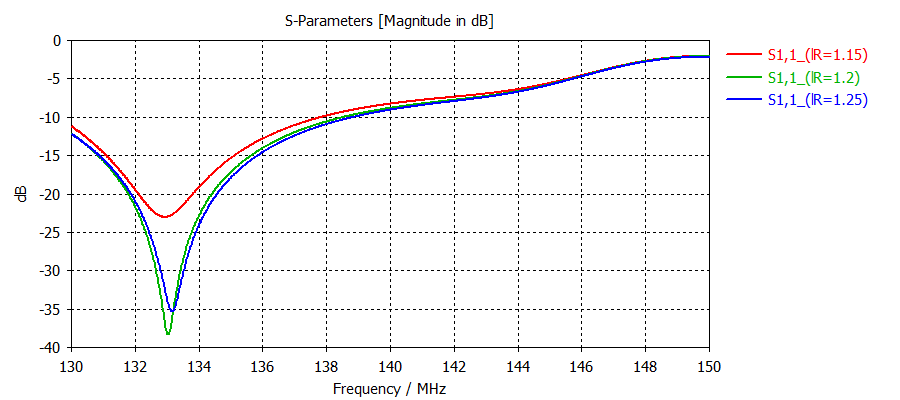
\includegraphics[width=\textwidth]{lR.png}
	\caption{Resultat durch Abändern der Reflektorlänge.}
	\label{fig:Simulation_lR}
\end{figure}

Wie im Kapitel \ref{sec:Berechnung} beschrieben soll die Länge des Reflektors mindestens eine halbe Wellenlänge betragen. Dieser Wert wurde grosszügig gerundet, wobei Abbildung \ref{fig:Simulation_lR} zu entnehmen ist, dass zu kleine Werte für die Reflektorlänge dem Antennengewinn viel mehr schaden als zu grosse Werte. Daher lohnt es sich, die Yagi-Antenne eher zu überdimensioneren anstelle von zu knappen Werten, damit der Antennengewinn nicht zu schwach ist. Jedoch muss dabei auch beachtet werden, dass ein zu langer Reflektor wiederum den Antennengewinn verschlechtern kann. Daher muss bei einem genauen Design ein Optimum gefunden werden.

\begin{figure}[h!]
	\centering
	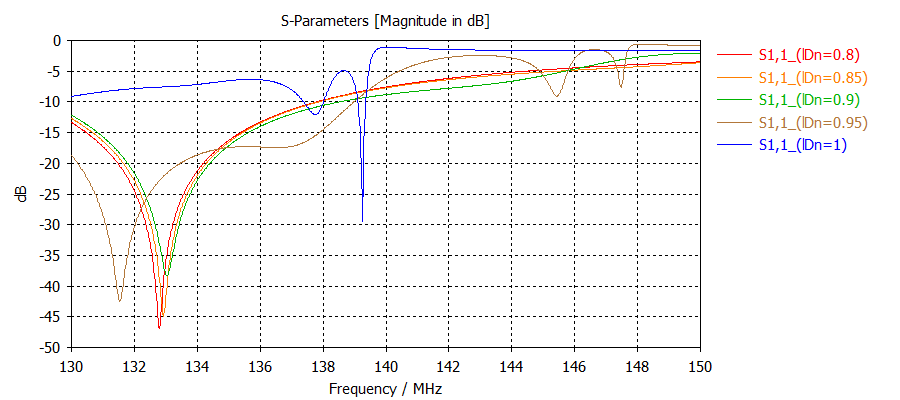
\includegraphics[width=\textwidth]{lDn.png}
	\caption{Einfluss der Direktorenlänge auf die S1,1 Parameter.}
	\label{fig:Simulation_lDn}
\end{figure}

Der Einfluss der Direktorenlänge ist in Abbildung \ref{fig:Simulation_lDn} zu sehen. Diese soll, wie in den Berechnungen beschrieben, weniger als eine halbe Wellenlänge betragen. Dabei scheinen zu knapp dimensionerte Werte sehr merkwürdige Resultate abzuliefern, weshalb bei dieser Simulation zwei zusätzliche Messungen durchgeführt wurden (eine Direktorenlänge von \SI{1}{m} beträgt weniger als eine halbe Wellenlänge, liefert jedoch schon zu schlechte Resultate). Bei kürzeren Direktoren wird nicht viel Antennengewinn aufgegeben, während für lange Werte die Grenzfrequenz stark verschoben wird (für die Messung mit dem längsten Reflektor liegt diese ausserhalb des gemessenen Bereiches). Daher lohnt es sich, diese eher zu kurz zu wählen.

\begin{figure}[h!]
	\centering
	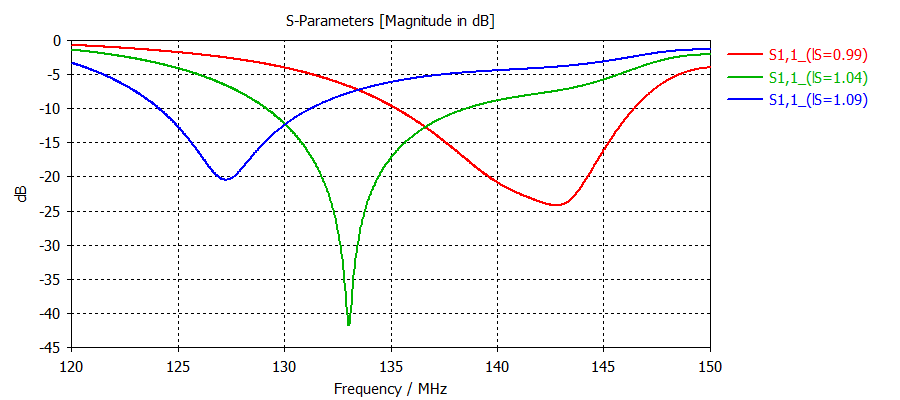
\includegraphics[width=\textwidth]{lS.png}
	\caption{Verhalten der S1,1 Parameter bei Abändern der Länge des Strahlers.}
	\label{fig:Simulation_lS}
\end{figure}

Abbildung \ref{fig:Simulation_lS} zeigt wie sich die Grenzfrequenz beim Abändern der Strahlerlänge verhält. Idealerweise beträgt diese Länge exakt eine halbe Wellenlänge, jedoch hat die Simulation gezeigt, dass die Grenzfrequenz der berechneten Antenne ungefähr \SI{10}{MHz} zu tief liegt. Diese Simulation zeigt jedoch, dass die Dimensionierung für die berechnete Antenne sich am Besten verhält im Gegensatz zu den anderen zwei Simulationen. Für kürzere oder längere Strahler kann die Grenzfrequenz im Gegensatz zu den vorherigen Messungen am effektivsten verschoben werden, jedoch leidet der Antennengewinn stark darunter.

\begin{figure}[h!]
	\centering
	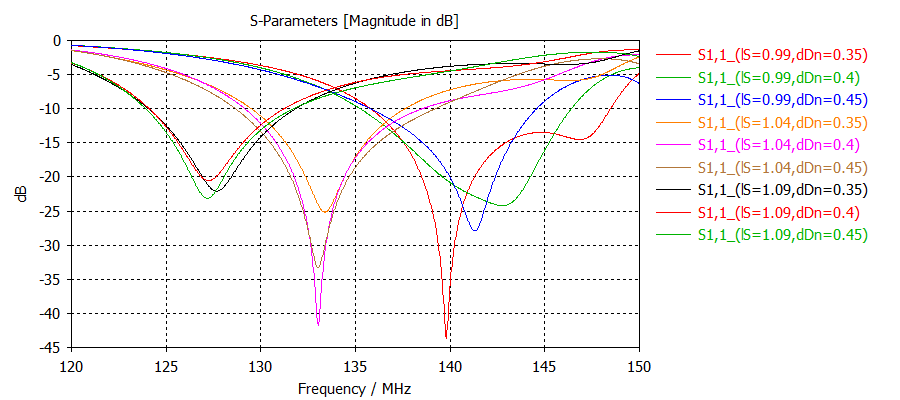
\includegraphics[width=\textwidth]{lS_dDn.png}
	\caption{Einfluss der Abänderung der Strahlerlänge und des Direktorenabstandes auf die S1,1 Parameter.}
	\label{fig:Simulation_lS_dDn}
\end{figure}

Anhand der vorherigen Simulation kann angenommen werden, dass bloss ein Abändern der Strahlerlänge nicht ausreicht. Deshalb wurde als Beispiel eine weitere Grösse angepasst. In Abbildung \ref{fig:Simulation_lS_dDn} sind die S1,1 Parameter zu sehen bei Veränderung der Strahlerlänge und der Direktorenabstände. Dabei wird zum Beispiel aufgezeigt, dass bei einem kürzeren Strahler durch das Anpassen der Direktorenabstände der Antennengewinn stark verbessert werden kann. Somit wurde durch die Simulation ein Parameterset gefunden, für welches die Antenne bei \SI{140}{MHz} sehr gute Eigenschaften besitzt. Dieses Verfahren könnte weiter verwendet werden, um ein Optimum bei \SI{144}{MHz} zu erreichen, was bei 5 veränderbaren Grössen relativ kompliziert werden kann. Da jedoch ein Grossteil der Simulationen bereits optimale Eigenschaften bei \SI{133}{MHz} aufweisen, wurden für den Bau der Antenne die bereits berechneten Werte verwendet.
